\chapter{Cloud storage}
After going through CPU and network virtualization, it's time to talk about
proper ways of handling storaged data. In the age of \emph{cloud computing}
there's a huge amount of data to store, access and secure, so novel approches
to system design are necessary. To achieve the goal of cloud computation,
effective data replication and appropriate storage management strategies are
critical.

In the past, storage system were desing according to a
\emph{performance-at-any-cost} philosophy, but now there's been a shift towards
\emph{reliability-at-the-lowest-possible-cost}. For example, data replication
allows concurrent access to data from multiple processors and decreases the
chances of data loss, but maintaining consistency among multiple copies of data
records increases the data management software complexity and could negatively
affect the storage system performance if data is frequently updated.

So, in this chapter we're going to explain some modern strategies adopted
to manage cloud storage while also respecting performance and realibility
requirements.

\section{Preliminary definitions}
Before proceding, we need to fix some concepts.

\begin{definition}[Storage model]
    A storage model describes the layout of a data structure in a physical storage.
\end{definition}
\begin{definition}[Data model]
    A data model captures the most important logical aspects of a data structure
    in a database
\end{definition}

\begin{definition}[Read-write coherence]
    The result of reading of a memory cell, should be the same as the most recent
    writing done on that cell.
\end{definition}
\begin{definition}[Before-or-after atomicity]
    The result of every read or write operation is the same as if that
    operation has been performed completely before or after another read or
    write operation.
\end{definition}

\noindent
\emph{Read-write coherenct} and \emph{Before-or-after atomicity} are two highly
desirable properties of any \emph{storage model}.

\subsection{Types of storage}
There are three main types of storage:
\begin{enumerate}
    \item \emph{Block storage}: data is managed as blocks within sectors and
    tracks. Can be used when storage has access to raw and unformatted hardware
    and is usedfull when both speed and efficiency are important;
    \item \emph{File storage}: data is organized as structured files which are
    managed through a file system. However, this doesn't work very well with
    large amounts of data or high-demands for a particular piece of data;
    \item \emph{Object storage}: data is managed as objects. Typically, each
    object has a gloabal unique identifier and holds both the data itself and
    some metadata. It's possible to access whole objects or blobs of data, but
    random access to data within an object is more difficult;
\end{enumerate}

\noindent
\emph{Block storage} is often used for database because it's the ideal way of
storing relational information. On the other hand, \emph{Object storage} isn't
suitable for databases, but is preferable to store content that can grow without
bounds, for example, backups and archives. Finally, the \emph{File storage} model
can be easily used to create \emph{distributed file system} vian network protocols.

Examples of \emph{Block storage}, \emph{File storage} and \emph{Object storage}
are, respectivelly, Cinder, Google file system and OpenStack Swift.

\section{Block storage}
We'll give a quick look to this model by scratching the surface of \emph{OpenStack
Cinder}. \emph{OpenStack Cinder} implements services and libraries to provide
on-demand, self-service access to block storage resources. It provides API to
interact with storage backends which is also exposed to the cloud. End users can
manage their storage without knowing how it's organized and for both physical and
virtual environments.

\begin{figure}[h!]
    \centering
    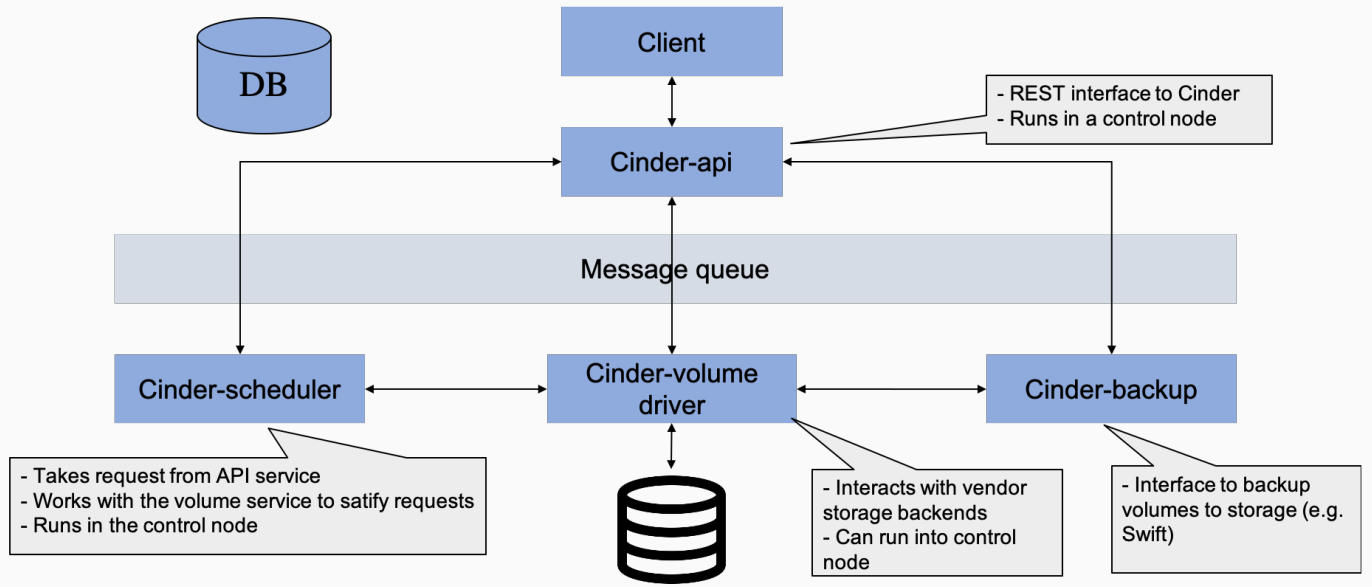
\includegraphics[width=0.7\textwidth]{images/block-model-cinder.png}
    \caption{\emph{OpenStack Cinder basic architecture}}
\end{figure}

\noindent
\emph{Cinder} APIs allow users to create and delete volumes and snaphots (for
backup pourposes). Attach or detach volumes for the available storage, clone and
extend them, and so on.

\section{Distributed file system}